\documentclass{../includes/TechDoc}
\usepackage[T1]{fontenc}
\usepackage[utf8]{inputenc}
%\usepackage[pdftex]{graphicx}
\DeclareGraphicsRule{*}{mps}{*}{}
\documentclass[12pt]{article}
\usepackage[russian]{babel}
\usepackage[utf8]{inputenc}

\renewcommand{\cftsecleader}{\cftdotfill{\cftdotsep}}

\newcommand{\intro}[1]{
    \stepcounter{section}
    \section*{\hfillПРИЛОЖЕНИЕ \arabic{section}}
    \begin{center}
        \Large\bf{#1}
    \end{center}
    \markboth{\MakeUppercase{#1}}{}
    \addcontentsline{toc}{section}{Приложение \arabic{section}. #1}
}

\title{Мобильное приложение для сообщений о бытовых проблемах студентов в общежитии}
\author{Студент группы БПИ-194}{В. А. Анненков}
\academicTeacher{Доцент департамента программной инженерии факультета компьютерных наук}{Х. М. Салех}

\documentTitle{Пояснительная записка}
\documentCode{RU.17701729.02.07-01 81 01-1}

\begin{document}
    \maketitle

    \begin{abstract}
        В данном программном документе приведена пояснительная записка к мобильному приложению <<Мобильное приложение для сообщений о бытовых проблемах студентов в общежитии>>.

        В данный документ внесены разделы «Введение», «Назначение и область применения программы», «Технические характеристики», «Ожидаемые технико-экономические показатели», «Источники, использованные при разработке».

        В разделе «Введение» указано наименование программы и документы, на основании которых ведется разработка.

        В разделе «Назначение и область применения» указано функциональное назначение программы и эксплуатационное назначение программы.

        В разделе «Технические характеристики» указаны постановка задачи на разработку программы, описание и обоснование метода организации входных и выходных данных, описание и обоснование выбора состава технических и программных средств.

        В разделе «Ожидаемые технико-экономические показатели» указана предполагаемая потребность и экономические преимущества разработки по сравнению с отечественными и зарубежными образцами или аналогами

        Настоящий документ разработан в соответствии с требованиями:
        \begin{enumerate}
            \item ГОСТ 19.101-77 Виды программ и программных документов [3];
            \item ГОСТ 19.102-77 Стадии разработки [4];
            \item ГОСТ 19.103-77 Обозначения программ и программных документов [5];
            \item ГОСТ 19.104-78 Основные надписи [6];
            \item ГОСТ 19.105-78 Общие требования к программным документам [7];
            \item ГОСТ 19.106-78 Требования к программным документам, выполненным печатным способом [8];
            \item ГОСТ 19.404-79 Пояснительная записка.
            Требования к содержанию и оформлению [9].
        \end{enumerate}
        Изменения к Пояснительной записке оформляются согласно ГОСТ 19.603-78 [10], ГОСТ 19.604-78 [11].
    \end{abstract}

    \newpage

    \tableofcontents


    \section{Введение}

    \subsection{Наименование программы}

    \subsubsection{Наименование программы на русском языке}

    Мобильное приложение для сообщений о бытовых проблемах студентов в общежитии.

    \subsubsection{Наименование программы на английском языке}

    Mobile Application for Informing about Household Problems in Dormitory.

    \subsection{Основание для разработки}

    Приказ декана факультета компьютерных наук И.В. Аржанцева "Об утверждении тем, руководителей курсовых работ студентов образовательной программы <<Программная инженерия>> факультета компьютерных наук" № 2.3-02/1112-04 от 11.12.2019.


    \section{Назначение и область применения}

    \subsection{Функциональное назначение}

    Функциональным назначением программы является помощь и консультирование студентов по вопросам, связанным
    с проживанием в общежитии.

    Студент может задать вопрос агенту поддержки, пообщаться в общем чате с другими
    студентами из этого же общежития, узнать последние новости общежития.

    Агент поддержки имеет доступ к панели администрирования, через которую он может создавать объявления, модерировать пользователей и их действия.
    Отвечать на обращения пользователей агент поддержки может с помощью мобильного приложения.

    Администратор имеет доступ к любым параметрам и данным в системе.

    \subsection{Эксплуатационное назначение}

    Программа может быть использована высшим учебным заведением для обеспечения централизованной связи со студентами, а
    также для информирования студентов о последних новостях в своих общежитиях.


    \section{Технические характеристики}

    \subsection{Постановка задачи}

    Программа должна обеспечивать возможность выполнения следующих функций:\\

    Для клиента:
    \begin{enumerate}[noitemsep]
        \item регистрация и авторизация;
        \item просмотр страницы с новостями;
        \item просмотр и редактирование собственного профиля;
        \item просмотр/создание/удаление/дополнение своих обращений;
        \item просмотр и взаимодействие с общим чатом.
    \end{enumerate}

    Для агента поддержки:
    \begin{enumerate}[noitemsep]
        \item регистрация и авторизация в приложении;
        \item регистрация и авторизация в панели администрирования;
        \item просмотр и изменение списка новостей;
        \item просмотр/изменение/удаление/дополнение любых обращений.
    \end{enumerate}

    Для администратора:
    \begin{enumerate}[noitemsep]
        \item всё, что доступно агенту поддержки;
        \item управление существующими агентами поддержки;
        \item возможность назначить или отозвать у пользователя статус агента поддержки;
        \item полный доступ без ограничений к панели администрирования.
    \end{enumerate}

    \begin{figure}[h]
        \centering
        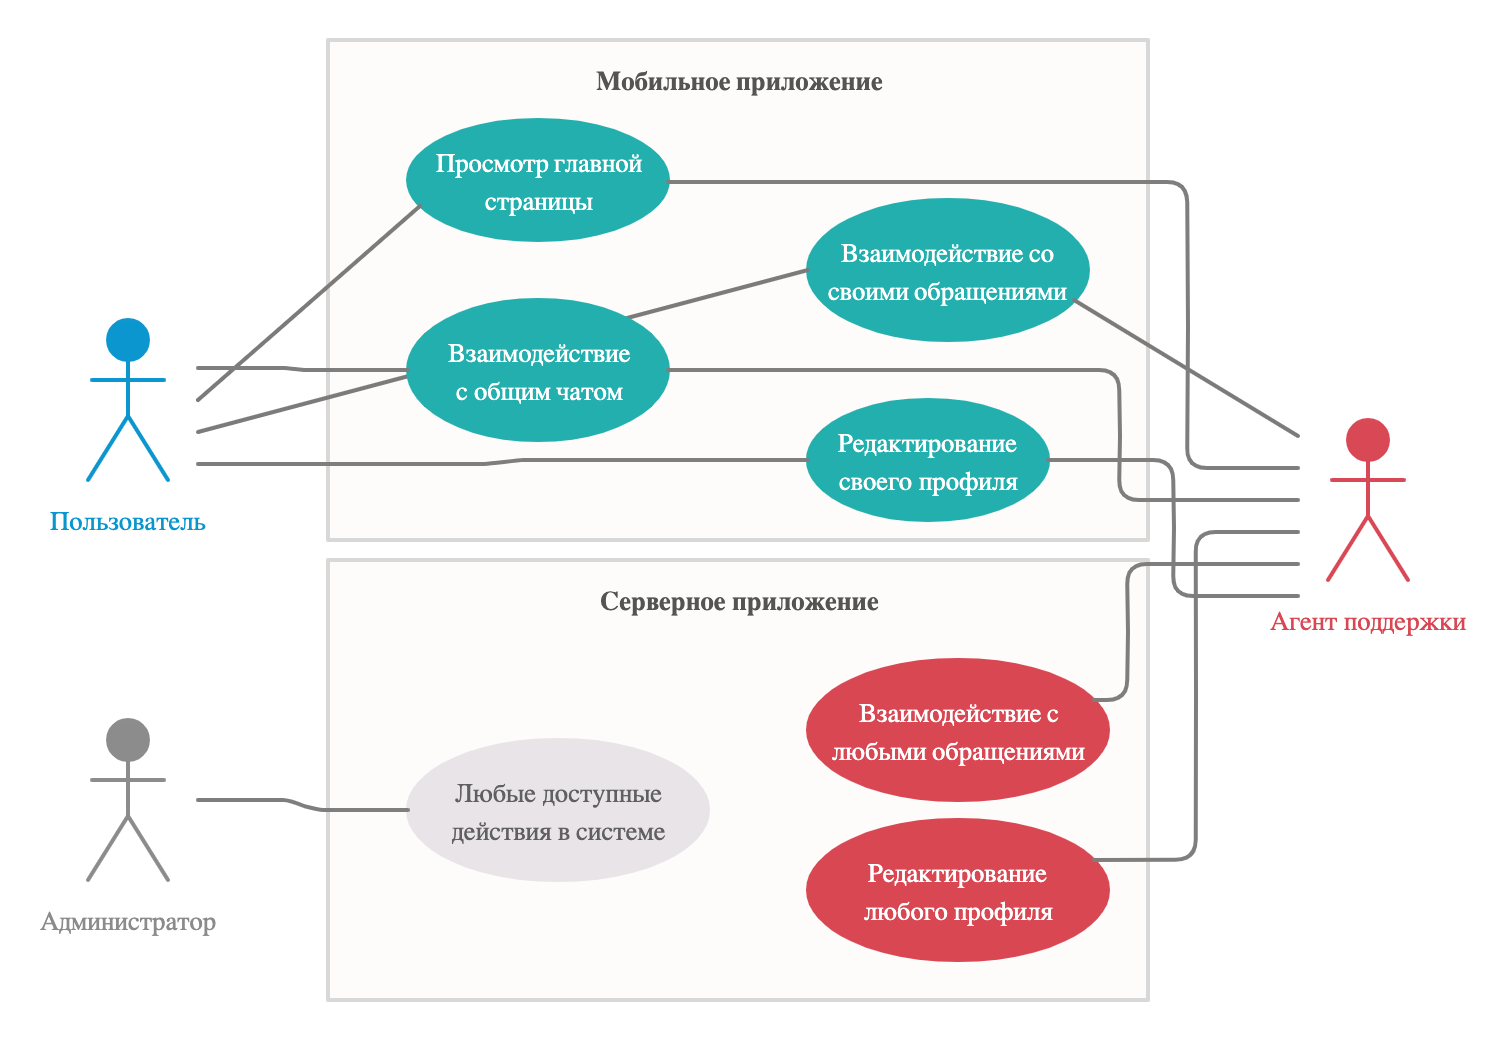
\includegraphics[width=0.8\linewidth]{images/uml_pr.png}
        \caption{Диаграмма прецедентов}
        \label{fig:uml_pr}
    \end{figure}

    \newpage

    \subsection{Описание алгоритма и функционирования программы}

    \subsubsection{Описание алгоритма и функционирования мобильного приложения}

    При первом запуске программы пользователю требуется авторизоваться в системе.
    Алгоритм авторизации следующий:
    \begin{enumerate}
        \item Пользователь вводит Email в домене @hse.ru или @edu.hse.ru.
        \item Система отправляет защитный код на указанный Email или возвращает ошибку, если был введён Email в стороннем домене.
        \item Пользователь вводит защитный код в соответствующее поле.
        \item Если пользователь авторизуется в системе впервые, приложение предложит заполнить профиль.
        В профиле содержатся следующие поля:
        \begin{enumerate}
            \item общежитие — общежитие, в котором проживает пользователь;
            \item комната — комната, в которой проживает пользователь.
        \end{enumerate}
    \end{enumerate}

    После авторизации пользователь попадает на главный экран.
    Меню для перехода между экранами расположено в нижней части экрана (Рис.~\ref{ris:menu}).

    \begin{figure}[ht]
        \centering
        \frame{
\includegraphics[width=0.8\linewidth]{images/menu.png}}
        \caption{Главное меню управления экранами приложения}
        \label{ris:menu}
    \end{figure}

    Описание функционала каждого экрана:
    \begin{enumerate}
        \item Экран <<Главная>> представляет собой главную страницу со следующими элементами:
        \begin{enumerate}
            \item общая информация профиля;
            \item новости;
            \item важные новости;
            \item предстоящие события;
            \item главные вопросы.
        \end{enumerate}

        \item Экран <<Профиль>>, на который можно попасть через главный экран, представляет собой форму с данными пользователя с возможностью редактирования;
        \item Экран <<Обращения>> представляет собой список обращений пользователя.
        \item Экран <<Обращение>> представляет собой страничку отдельного обращения со следующими элементами:
        \begin{enumerate}
            \item заголовок проблемы;
            \item описание;
            \item переписка пользователя с агентом поддержки.
        \end{enumerate}
        \item Экран <<Беседа>> представляет собой общий чат конкретного общежития;
        \item Экран <<О приложении>> представляет собой страницу с описанием приложения;
    \end{enumerate}

    \subsubsection{Описание алгоритма и функционирования серверного приложения}

    \paragraph{Общее описание}

    Взаимодействие с серверным приложением производится с помощью HTTP-запросов.
    Каждый запрос, кроме запросов авторизации, требует передачи токена, по которому идентифицируется пользователь.
    Токен передаётся в Header с ключом <<Authorization>> и значением <<Token \ldots>>, где на месте многоточия
    отправляется токен пользователя.\\

    Методы поддерживают следующие типы запросов:
    \begin{enumerate}
        \item GET — тип запроса для получения информации.
        Дополнительные параметры передаются с помощью query string, т.е. параметры передаются через адрес запроса
        следующим образом: <<https://url.ru/method?\textbf{param1=value1&param2=value2}>>.
        \item POST — тип запроса для добавления/изменения информации.
        Дополнительные параметры передаются в теле запроса.
        \item DELETE — тип запроса для удаления информации.
        Дополнительные параметры передаются в теле запроса.
    \end{enumerate}\\

    \paragraph{Описание методов серверного приложения}
    В скобках указаны параметры, которые требуют методы.
    \begin{enumerate}
        \item Метод <</auth/register>> отправляет защитный код на почту.\\
        Поддерживаемые типы запросов:
        \begin{enumerate}
            \item POST (email)\@.
        \end{enumerate}
        \item Метод <</auth/register/confirm-email>> проверяет указанный защитный код с отправленным ранее на почту.\\
        Поддерживаемые типы запросов:
        \begin{enumerate}
            \item POST (email, code)\@.
        \end{enumerate}
        \item Метод <</main\_page>> позволяет получить информацию с главной страницы.\\
        Поддерживаемые типы запросов:
        \begin{enumerate}
            \item GET\@.
        \end{enumerate}
        \item Метод <</profile>> позволяет получить информацию о своём профиле.\\
        Поддерживаемые типы запросов:
        \begin{enumerate}
            \item GET\@;
            \item POST (dormitory, room)\@.
        \end{enumerate}
        \item Метод <</dormitories>> позволяет взаимодействовать с моделями общежитий.\\
        Поддерживаемые типы запросов:
        \begin{enumerate}
            \item GET\@.
        \end{enumerate}
        \item Метод <</problems>> позволяет взаимодействовать с моделями обращений.
        Поддерживаемые типы запросов:
        \begin{enumerate}
            \item GET\@;
            \item POST (id, title, description, status) — для агентов поддержки;
            \item DELETE (id) — для агентов поддержки.
        \end{enumerate}
        \item Метод <</messages>> позволяет взаимодействовать с моделями сообщений.\\
        Поддерживаемые типы запросов:
        \begin{enumerate}
            \item GET\@;
            \item POST (id, text)\@.
        \end{enumerate}
        \item Метод <</notices>> позволяет взаимодействовать с моделями новостей.
        Поддерживаемые типы запросов:
        \begin{enumerate}
            \item GET\@;
            \item POST (id, title, text) — для агентов поддержки.
            \item DELETE (id) — для агентов поддержки.
        \end{enumerate}
    \end{enumerate}

    \clearpage

    \subsection{Описание и обоснование метода организации входных и выходных данных}

    \subsubsection{Описание и обоснование метода организации входных и выходных данных мобильного приложения}

    Входные данные вводятся пользователем вручную в соответствующие для этого текстовые поля или путём нажатия на кнопки интерфейса.

    Выходные данные отображаются в виде текста и иконок.

    \subsubsection{Описание и обоснование метода организации входных и выходных данных серверного приложения}

    Входные данные предоставляются в виде GET/POST/DELETE запросов с дополнительными параметрами.

    Выходные данные предоставляются в виде JSON-модели в качестве ответа на запрос.

    Такой подход позволяет эффективно выстраивать модель взаимодействия мобильного приложения с сервером.
    Также с помощью такого подхода можно передать информацию практически любого формата: число, текст, дату, картинку и т.д.\\

    \noindent\textbf{Пример запроса:}

    \noindentОтправлен корректный запрос на адрес \url{https://hse-supporter.herokuapp.com/profile};\\

    \noindentПолучен ответ:
    \begin{lstlisting}
    {
        "id": 1,
        "first_name": "Vladislav",
        "last_name": "Annenkov",
        "role": "agent",
        "room": "#100",
        "dormitory": {
        "id": 10,
        "name": "Dormitory №8",
        "address": "Odintsovo, st. Makovsky, d. 2"
    },
    "additional_info": {
        "dormitory_users_count": 3,
        "agents_online_count": 1
    }
    }
    \end{lstlisting}

    \clearpage

    \subsection{Описание и обоснование выбора состава технических и программных средств}

    \subsubsection{Состав технических и программных средств}

    Для работы программы необходим следующий набор программных средств:
    \begin{itemize}
        \item ОС iOS 8 или выше.
    \end{itemize}

    Для работы программы необходим следующий набор технических средств:
    \begin{itemize}
        \item сенсорный экран;
        \item стабильное интернет-подключение;
        \item не менее 512MB оперативной памяти;
        \item не менее 50 МБ свободной памяти на устройстве.
    \end{itemize}

    \subsubsection{Обоснование выбора состава технических и программных средств}

    В качестве реализации мобильного приложения были выбраны язык программирования C\# и фреймворк Xamarin.
    Это позволило пользоваться обширной библиотекой пакетов NuGet.

    В качестве реализации серверной части были выбраны язык программирования Python и веб-фреймворк Django.
    Это позволило ускорить процесс разработки за счёт использования вспомогательных библиотек.

    Как дополнительный фреймворк для реализации REST API был использован <<Django REST framework>>.
    Данный фреймворк позволяет гибко настроить взаимодействие с моделями базы данных через REST API\@.

    В качестве сервиса для деплоя серверной части был выбран веб-сервис Heroku.
    Это позволило гибко настроить базу данных и подключить автоматический деплой после каждого коммита в ветке master.

    Для работы с API была выбрана библиотека Refit.
    Это бесплатная библиотека, которая которая позволяет описать способ взаимодействия с REST API методами через
    интерфейсы в языке C\#.
    Данный подход ускоряет процесс разработки.

    В качестве СУБД была выбрана система PostgreSQL\@.
    Такое решение было принято по нескольким причинам:
    \begin{enumerate}
        \item открытый исходный код СУБД, что делает её бесплатной;
        \item адаптированность для хранения и обработки больших объёмов данных;
        \item хорошая поддержка фреймворком Django;
        \item возможность подключить PostgreSQL в админ-панели Heroku.
    \end{enumerate}


    \section{Ожидаемые технико-экономические показатели}

    \subsection{Предполагаемая потребность}

    Мобильное приложение могут использовать образовательные организации для централизованной связи со студентами своих
    общежитий.

    \subsection{Экономические преимущества по сравнению с отечественными и зарубежными аналогами}

    На момент начала разработки на рынке не было выявлено аналогичных продуктов.

    \clearpage


    \section{Источники, использованные при разработке}

    \begin{enumerate}
        \item Единая система программной документации – М.: ИПК, Издательство стандартов, 2000, 125 стр.
        \item LMS [Электронный ресурс] URL: \url{https://lms.hse.ru/} (Дата обращения: 30.04.2020, режим доступа: свободный)
        \item РУЗ [Электронный ресурс] URL: \url{https://ruz.hse.ru/} (Дата обращения: 30.04.2020, режим доступа: свободный)
        \item GitHub [Электронный ресурс] URL: \url{https://github.com/} (Дата обращения: 30.04.2020, режим доступа: свободный)
        \item Документация Microsoft [Электронный справочник] URL: \url{https://docs.microsoft.com/ru-ru/} (Дата обращения: 30.04.2020, режим доступа: свободный)
        \item StackOverflow [Электронный ресурс] URL: \url{https://stackoverflow.com/} (Дата обращения: 30.04.2020, режим доступа: свободный)
    \end{enumerate}

    \clearpage
    \appendix

    \intro{Терминология}

    \noindent
    \textbf{Агент поддержки} — пользователь с доступом к панели администрирования и обращениям всех пользователей.\\\\
    \textbf{Администратор} — пользователь с доступом к любым настройкам панели администрирования.\\\\
    \textbf{Деплой} — удалённый запуск серверного приложения.\\\\
    \textbf{Защитный код} — набор латинских символов и цифр определённой длины.\\\\
    \textbf{Сервер} — выделенный или специализированный компьютер для выполнения сервисного программного обеспечения.\\\\
    \textbf{Серверное приложение} — программа на сервере.\\\\
    \textbf{СУБД} — система управления базами данных.\\\\
    \textbf{Фреймворк} — дополнение к программе, расширяющее функционал или упрощающее процесс разработки.\\\\

    \intro{Структура базы данных}

    Приведена схема базы данных (Рис.~\ref{fig:api_scheme}).

    В базе данных:
    \begin{itemize}[noitemsep]
        \item таблица auth\_user хранит основную информацию о пользователях;
        \item таблица api\_profile хранит информацию профилей пользователей;
        \item таблица auth\_group хранит пользовательские группы;
        \item таблица auth\_user\_groups хранит группы, к которым принадлежат пользователи;
        \item таблица authtoken\_token хранит токены для авторизации;
        \item таблица auth\_permission хранит информацию о разрешениях;
        \item таблица auth\_group\_permissions хранит разрешения для каждой группы;
        \item таблица auth\_user\_user\_permissions хранит разрешения для каждого пользователя;
        \item таблица api\_dormitory хранит информацию об общежитиях;
        \item таблица api\_problem хранит информацию об обращениях пользователей;
        \item таблица api\_message хранит информацию о сообщениях к обращениям и в общих чатах;
        \item таблица api\_notice хранит информацию о новостях на главной странице;
        \item таблица api\_event хранит информацию о предстоящих событиях.
    \end{itemize}

    \begin{figure}[h]
        \centering
        \frame{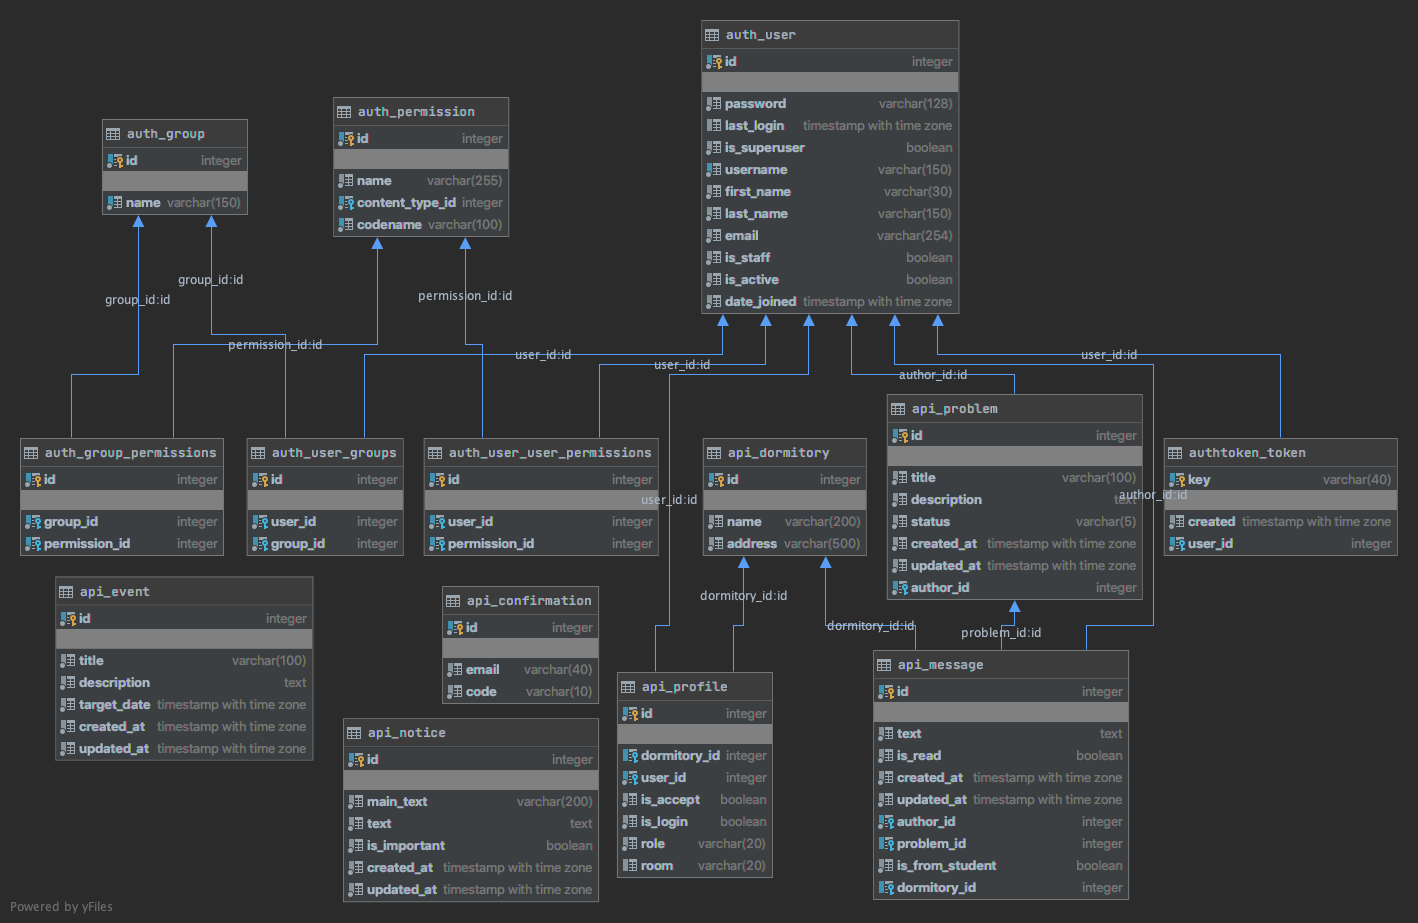
\includegraphics[width=1\linewidth]{images/api_scheme.png}}
        \caption{Схема облачного хранилища}
        \label{fig:api_scheme}
    \end{figure}

    \intro{Описание классов, структур, методов, полей серверного приложения}

    \begin{table}[ht]
        \caption{\label{tab:classes-table-server}Функциональное назначение классов серверного приложения.}
        \centering
        \begin{tabular}{ | p{4.5cm} | p{12.5cm} | }
            \hline
            \textbf{Класс} & \textbf{Назначение}  \\ \hline
            AuthView & Отправляет защитный код на почту \\ \hline
            AuthConfirmView & Проверяет указанный защитный код с отправленным ранее на почту \\ \hline
            ProfileView & Позволяет получить информацию о своём профиле \\ \hline
            MainPageView & Позволяет получить информацию с главной страницы \\ \hline
            DormitoriesViewSet & Позволяет взаимодействовать с моделями общежитий \\ \hline
            ProblemViewSet & Позволяет взаимодействовать с моделями обращений \\ \hline
            MessagesViewSet & Позволяет взаимодействовать с моделями сообщений \\ \hline
            NoticesViewSet & Позволяет взаимодействовать с моделями новостей \\ \hline
            Dormitory & Модель БД общежития \\ \hline
            Problem & Модель БД обращения \\ \hline
            Message & Модель БД сообщения \\ \hline
            Notice & Модель БД новости \\ \hline
            Event & Модель БД предстоящего события \\ \hline
            Profile & Модель БД профиля \\ \hline
            Confirmation & Модель БД кода подтверждения \\ \hline
            UserSerializer & Сериализатор модели пользователя \\ \hline
            DormitorySerializer & Сериализатор модели общежития \\ \hline
            ProblemSerializer & Сериализатор модели обращения \\ \hline
            MessageSerializer & Сериализатор модели сообщения \\ \hline
            NoticeSerializer & Сериализатор модели новости \\ \hline
            EventSerializer & Сериализатор модели предстоящего события \\ \hline
        \end{tabular}
    \end{table}

    \intro{Описание и функциональное назначение полей, методов и свойств серверного приложения}

    \begin{table}[ht]
        \caption{\label{tab:class-AuthView-table}Описание полей, методов и свойств класса AuthView}
        \centering
        \begin{tabular}{|p{3.2cm}|p{3cm}|p{2.9cm}|p{2.9cm}|p{4cm}|}
            \hline
            \multicolumn{5}{|c|}{AuthView} \\ \hline
            \multicolumn{5}{|l|}{\textbf{Методы}} \\ \hline
            \textbf{Имя} & \textbf{Модификатор доступа} & \textbf{Тип} & \textbf{Аргументы} & \textbf{Назначение} \\ \hline
            post & public & Response & request & Реализация POST-запроса для метода отправки кода подтверждения \\ \hline
        \end{tabular}
    \end{table}

    \begin{table}[ht]
        \caption{\label{tab:class-AuthConfirmView-table}Описание полей, методов и свойств класса AuthConfirmView}
        \centering
        \begin{tabular}{|p{3.2cm}|p{3cm}|p{2.9cm}|p{2.9cm}|p{4cm}|}
            \hline
            \multicolumn{5}{|c|}{AuthConfirmView} \\ \hline
            \multicolumn{5}{|l|}{\textbf{Методы}} \\ \hline
            \textbf{Имя} & \textbf{Модификатор доступа} & \textbf{Тип} & \textbf{Аргументы} & \textbf{Назначение} \\ \hline
            post & public & Response & request & Реализация POST-запроса для метода авторизации \\ \hline
        \end{tabular}
    \end{table}

    \begin{table}[ht]
        \caption{\label{tab:class-ProfileView-table}Описание полей, методов и свойств класса ProfileView}
        \centering
        \begin{tabular}{|p{3.2cm}|p{3cm}|p{2.9cm}|p{2.9cm}|p{4cm}|}
            \hline
            \multicolumn{5}{|c|}{ProfileView} \\ \hline
            \multicolumn{5}{|l|}{\textbf{Методы}} \\ \hline
            \textbf{Имя} & \textbf{Модификатор доступа} & \textbf{Тип} & \textbf{Аргументы} & \textbf{Назначение} \\ \hline
            get & public & Response & request & Реализация GET-запроса для метода профиля \\ \hline
            post & public & Response & request & Реализация POST-запроса для метода профиля \\ \hline
        \end{tabular}
    \end{table}

    \begin{table}[ht]
        \caption{\label{tab:class-MainPageView-table}Описание полей, методов и свойств класса MainPageView}
        \centering
        \begin{tabular}{|p{3.2cm}|p{3cm}|p{2.9cm}|p{2.9cm}|p{4cm}|}
            \hline
            \multicolumn{5}{|c|}{MainPageView} \\ \hline
            \multicolumn{5}{|l|}{\textbf{Методы}} \\ \hline
            \textbf{Имя} & \textbf{Модификатор доступа} & \textbf{Тип} & \textbf{Аргументы} & \textbf{Назначение} \\ \hline
            get & public & Response & request & Реализация GET-запроса для метода главной страницы \\ \hline
        \end{tabular}
    \end{table}

    \begin{table}[ht]
        \caption{\label{tab:class-DormitoriesViewSet-table}Описание полей, методов и свойств класса DormitoriesViewSet}
        \centering
        \begin{tabular}{|p{3.2cm}|p{3cm}|p{2.9cm}|p{2.9cm}|p{4cm}|}
            \hline
            \multicolumn{5}{|c|}{DormitoriesViewSet} \\ \hline
            \multicolumn{5}{|l|}{\textbf{Поля}} \\ \hline
            \textbf{Имя} & \textbf{Модификатор доступа} & \textbf{Тип} & \multicolumn{2}{p{6.9cm}|}{\textbf{Описание}} \\ \hline
            serializer\_class & public & Dormitory Serializer & \multicolumn{2}{p{6.9cm}|}{Класс сериализации для метода} \\ \hline
            \multicolumn{5}{|l|}{\textbf{Методы}} \\ \hline
            \textbf{Имя} & \textbf{Модификатор доступа} & \textbf{Тип} & \textbf{Аргументы} & \textbf{Назначение} \\ \hline
            get\_queryset & public & objects & request & Получение списка общежитий для метода GET \\ \hline
            get & public & Response & request & Реализация GET-запроса для метода общежитий \\ \hline
        \end{tabular}
    \end{table}

    \begin{table}[ht]
        \caption{\label{tab:class-ProblemViewSet-table}Описание полей, методов и свойств класса ProblemViewSet}
        \centering
        \begin{tabular}{|p{3.2cm}|p{3cm}|p{2.9cm}|p{2.9cm}|p{4cm}|}
            \hline
            \multicolumn{5}{|c|}{ProblemViewSet} \\ \hline
            \multicolumn{5}{|l|}{\textbf{Поля}} \\ \hline
            \textbf{Имя} & \textbf{Модификатор доступа} & \textbf{Тип} & \multicolumn{2}{p{6.9cm}|}{\textbf{Описание}} \\ \hline
            serializer\_class & public & Problem Serializer & \multicolumn{2}{p{6.9cm}|}{Класс сериализации для метода} \\ \hline
            \multicolumn{5}{|l|}{\textbf{Методы}} \\ \hline
            \textbf{Имя} & \textbf{Модификатор доступа} & \textbf{Тип} & \textbf{Аргументы} & \textbf{Назначение} \\ \hline
            get\_queryset & public & objects & request & Получение списка обращений для метода GET \\ \hline
            get & public & Response & request & Реализация GET-запроса для метода обращений \\ \hline
            create & public & Response & request & Реализация POST-запроса для метода обращений \\ \hline
            destroy & public & Response & request & Реализация DELETE-запроса для метода обращений \\ \hline
        \end{tabular}
    \end{table}

    \begin{table}[ht]
        \caption{\label{tab:class-MessagesViewSet-table}Описание полей, методов и свойств класса MessagesViewSet}
        \centering
        \begin{tabular}{|p{3.2cm}|p{3cm}|p{2.9cm}|p{2.9cm}|p{4cm}|}
            \hline
            \multicolumn{5}{|c|}{MessagesViewSet} \\ \hline
            \multicolumn{5}{|l|}{\textbf{Поля}} \\ \hline
            \textbf{Имя} & \textbf{Модификатор доступа} & \textbf{Тип} & \multicolumn{2}{p{6.9cm}|}{\textbf{Описание}} \\ \hline
            serializer\_class & public & Message Serializer & \multicolumn{2}{p{6.9cm}|}{Класс сериализации для метода} \\ \hline
            \multicolumn{5}{|l|}{\textbf{Методы}} \\ \hline
            \textbf{Имя} & \textbf{Модификатор доступа} & \textbf{Тип} & \textbf{Аргументы} & \textbf{Назначение} \\ \hline
            get\_queryset & public & objects & request & Получение списка сообщений для метода GET \\ \hline
            get & public & Response & request & Реализация GET-запроса для метода сообщений \\ \hline
            create & public & Response & request & Реализация POST-запроса для метода сообщений \\ \hline
        \end{tabular}
    \end{table}

    \begin{table}[ht]
        \caption{\label{tab:class-NoticesViewSet-table}Описание полей, методов и свойств класса NoticesViewSet}
        \centering
        \begin{tabular}{|p{3.2cm}|p{3cm}|p{2.9cm}|p{2.9cm}|p{4cm}|}
            \hline
            \multicolumn{5}{|c|}{NoticesViewSet} \\ \hline
            \multicolumn{5}{|l|}{\textbf{Поля}} \\ \hline
            \textbf{Имя} & \textbf{Модификатор доступа} & \textbf{Тип} & \multicolumn{2}{p{6.9cm}|}{\textbf{Описание}} \\ \hline
            serializer\_class & public & Notice Serializer & \multicolumn{2}{p{6.9cm}|}{Класс сериализации для метода} \\ \hline
            \multicolumn{5}{|l|}{\textbf{Методы}} \\ \hline
            \textbf{Имя} & \textbf{Модификатор доступа} & \textbf{Тип} & \textbf{Аргументы} & \textbf{Назначение} \\ \hline
            get\_queryset & public & objects & request & Получение списка новостей для метода GET \\ \hline
            get & public & Response & request & Реализация GET-запроса для метода новостей \\ \hline
        \end{tabular}
    \end{table}

    \begin{table}[ht]
        \caption{\label{tab:class-Dormitory-table}Описание полей, методов и свойств класса Dormitory}
        \centering
        \begin{tabular}{|p{3.2cm}|p{3cm}|p{2.9cm}|p{2.9cm}|p{4cm}|}
            \hline
            \multicolumn{5}{|c|}{Dormitory} \\ \hline
            \multicolumn{5}{|l|}{\textbf{Классы}} \\ \hline
            \textbf{Имя} & \textbf{Модификатор доступа} & \multicolumn{3}{p{9.8cm}|}{\textbf{Описание}} \\ \hline
            Meta & public & \multicolumn{3}{p{9.8cm}|}{Класс с параметрами модели} \\ \hline
            \multicolumn{5}{|l|}{\textbf{Поля}} \\ \hline
            \textbf{Имя} & \textbf{Модификатор доступа} & \textbf{Тип} & \multicolumn{2}{p{6.9cm}|}{\textbf{Описание}} \\ \hline
            name & public & CharField & \multicolumn{2}{p{6.9cm}|}{Имя общежития} \\ \hline
            address & public & CharField & \multicolumn{2}{p{6.9cm}|}{Адрес общежития} \\ \hline
            \multicolumn{5}{|l|}{\textbf{Методы}} \\ \hline
            \textbf{Имя} & \textbf{Модификатор доступа} & \textbf{Тип} & \textbf{Аргументы} & \textbf{Назначение} \\ \hline
            \_\_str\_\_ & public & string & - & Строковое представление модели \\ \hline
        \end{tabular}
    \end{table}

    \begin{table}[ht]
        \caption{\label{tab:class-Problem-table}Описание полей, методов и свойств класса Problem}
        \centering
        \begin{tabular}{|p{3.2cm}|p{3cm}|p{2.9cm}|p{2.9cm}|p{4cm}|}
            \hline
            \multicolumn{5}{|c|}{Problem} \\ \hline
            \multicolumn{5}{|l|}{\textbf{Классы}} \\ \hline
            \textbf{Имя} & \textbf{Модификатор доступа} & \multicolumn{3}{p{9.8cm}|}{\textbf{Описание}} \\ \hline
            Status & public & \multicolumn{3}{p{9.8cm}|}{Класс с вариантами статуса обращения} \\ \hline
            Meta & public & \multicolumn{3}{p{9.8cm}|}{Класс с параметрами модели} \\ \hline
            \multicolumn{5}{|l|}{\textbf{Поля}} \\ \hline
            \textbf{Имя} & \textbf{Модификатор доступа} & \textbf{Тип} & \multicolumn{2}{p{6.9cm}|}{\textbf{Описание}} \\ \hline
            author & public & ForeignKey & \multicolumn{2}{p{6.9cm}|}{Автор обращения} \\ \hline
            title & public & CharField & \multicolumn{2}{p{6.9cm}|}{Заголовок обращения} \\ \hline
            description & public & TextField & \multicolumn{2}{p{6.9cm}|}{Описание обращения} \\ \hline
            status & public & CharField & \multicolumn{2}{p{6.9cm}|}{Статус обращения} \\ \hline
            created\_at & public & DateTimeField & \multicolumn{2}{p{6.9cm}|}{Дата создания обращения} \\ \hline
            updated\_at & public & DateTimeField & \multicolumn{2}{p{6.9cm}|}{Дата обновления обращения} \\ \hline
            \multicolumn{5}{|l|}{\textbf{Методы}} \\ \hline
            \textbf{Имя} & \textbf{Модификатор доступа} & \textbf{Тип} & \textbf{Аргументы} & \textbf{Назначение} \\ \hline
            \_\_str\_\_ & public & string & - & Строковое представление модели \\ \hline
        \end{tabular}
    \end{table}

    \begin{table}[ht]
        \caption{\label{tab:class-Message-table}Описание полей, методов и свойств класса Message}
        \centering
        \begin{tabular}{|p{3.2cm}|p{3cm}|p{2.9cm}|p{2.9cm}|p{4cm}|}
            \hline
            \multicolumn{5}{|c|}{Message} \\ \hline
            \multicolumn{5}{|l|}{\textbf{Классы}} \\ \hline
            \textbf{Имя} & \textbf{Модификатор доступа} & \multicolumn{3}{p{9.8cm}|}{\textbf{Описание}} \\ \hline
            Meta & public & \multicolumn{3}{p{9.8cm}|}{Класс с параметрами модели} \\ \hline
            \multicolumn{5}{|l|}{\textbf{Поля}} \\ \hline
            \textbf{Имя} & \textbf{Модификатор доступа} & \textbf{Тип} & \multicolumn{2}{p{6.9cm}|}{\textbf{Описание}} \\ \hline
            author & public & ForeignKey & \multicolumn{2}{p{6.9cm}|}{Автор сообщения} \\ \hline
            text & public & TextField & \multicolumn{2}{p{6.9cm}|}{Текст сообщения} \\ \hline
            problem & public & ForeignKey & \multicolumn{2}{p{6.9cm}|}{Обращение, к которому относится сообщение} \\ \hline
            dormitory & public & ForeignKey & \multicolumn{2}{p{6.9cm}|}{Общий чат общежития, к которому относится сообщение} \\ \hline
            created\_at & public & DateTimeField & \multicolumn{2}{p{6.9cm}|}{Дата создания обращения} \\ \hline
            updated\_at & public & DateTimeField & \multicolumn{2}{p{6.9cm}|}{Дата обновления обращения} \\ \hline
            \multicolumn{5}{|l|}{\textbf{Методы}} \\ \hline
            \textbf{Имя} & \textbf{Модификатор доступа} & \textbf{Тип} & \textbf{Аргументы} & \textbf{Назначение} \\ \hline
            \_\_str\_\_ & public & string & - & Строковое представление модели \\ \hline
        \end{tabular}
    \end{table}

    \begin{table}[ht]
        \caption{\label{tab:class-Notice-table}Описание полей, методов и свойств класса Notice}
        \centering
        \begin{tabular}{|p{3.2cm}|p{3cm}|p{2.9cm}|p{2.9cm}|p{4cm}|}
            \hline
            \multicolumn{5}{|c|}{Notice} \\ \hline
            \multicolumn{5}{|l|}{\textbf{Классы}} \\ \hline
            \textbf{Имя} & \textbf{Модификатор доступа} & \multicolumn{3}{p{9.8cm}|}{\textbf{Описание}} \\ \hline
            Meta & public & \multicolumn{3}{p{9.8cm}|}{Класс с параметрами модели} \\ \hline
            \multicolumn{5}{|l|}{\textbf{Поля}} \\ \hline
            \textbf{Имя} & \textbf{Модификатор доступа} & \textbf{Тип} & \multicolumn{2}{p{6.9cm}|}{\textbf{Описание}} \\ \hline
            main\_text & public & CharField & \multicolumn{2}{p{6.9cm}|}{Главный текст новости} \\ \hline
            text & public & TextField & \multicolumn{2}{p{6.9cm}|}{Подробный текст новости} \\ \hline
            is\_important & public & BooleanField & \multicolumn{2}{p{6.9cm}|}{Важная ли новость} \\ \hline
            created\_at & public & DateTimeField & \multicolumn{2}{p{6.9cm}|}{Дата создания обращения} \\ \hline
            updated\_at & public & DateTimeField & \multicolumn{2}{p{6.9cm}|}{Дата обновления обращения} \\ \hline
            \multicolumn{5}{|l|}{\textbf{Методы}} \\ \hline
            \textbf{Имя} & \textbf{Модификатор доступа} & \textbf{Тип} & \textbf{Аргументы} & \textbf{Назначение} \\ \hline
            \_\_str\_\_ & public & string & - & Строковое представление модели \\ \hline
        \end{tabular}
    \end{table}

    \begin{table}[ht]
        \caption{\label{tab:class-Event-table}Описание полей, методов и свойств класса Event}
        \centering
        \begin{tabular}{|p{3.2cm}|p{3cm}|p{2.9cm}|p{2.9cm}|p{4cm}|}
            \hline
            \multicolumn{5}{|c|}{Event} \\ \hline
            \multicolumn{5}{|l|}{\textbf{Классы}} \\ \hline
            \textbf{Имя} & \textbf{Модификатор доступа} & \multicolumn{3}{p{9.8cm}|}{\textbf{Описание}} \\ \hline
            Meta & public & \multicolumn{3}{p{9.8cm}|}{Класс с параметрами модели} \\ \hline
            \multicolumn{5}{|l|}{\textbf{Поля}} \\ \hline
            \textbf{Имя} & \textbf{Модификатор доступа} & \textbf{Тип} & \multicolumn{2}{p{6.9cm}|}{\textbf{Описание}} \\ \hline
            title & public & CharField & \multicolumn{2}{p{6.9cm}|}{Заголовок события} \\ \hline
            description & public & TextField & \multicolumn{2}{p{6.9cm}|}{Описание события} \\ \hline
            target\_date & public & DateTimeField & \multicolumn{2}{p{6.9cm}|}{Дата проведения события} \\ \hline
            created\_at & public & DateTimeField & \multicolumn{2}{p{6.9cm}|}{Дата создания обращения} \\ \hline
            updated\_at & public & DateTimeField & \multicolumn{2}{p{6.9cm}|}{Дата обновления обращения} \\ \hline
            \multicolumn{5}{|l|}{\textbf{Методы}} \\ \hline
            \textbf{Имя} & \textbf{Модификатор доступа} & \textbf{Тип} & \textbf{Аргументы} & \textbf{Назначение} \\ \hline
            \_\_str\_\_ & public & string & - & Строковое представление модели \\ \hline
        \end{tabular}
    \end{table}

    \begin{table}[ht]
        \caption{\label{tab:class-Profile-table}Описание полей, методов и свойств класса Profile}
        \centering
        \begin{tabular}{|p{3.2cm}|p{3cm}|p{2.9cm}|p{2.9cm}|p{4cm}|}
            \hline
            \multicolumn{5}{|c|}{Profile} \\ \hline
            \multicolumn{5}{|l|}{\textbf{Классы}} \\ \hline
            \textbf{Имя} & \textbf{Модификатор доступа} & \multicolumn{3}{p{9.8cm}|}{\textbf{Описание}} \\ \hline
            Role & public & \multicolumn{3}{p{9.8cm}|}{Класс с вариантами роли профиля} \\ \hline
            Meta & public & \multicolumn{3}{p{9.8cm}|}{Класс с параметрами модели} \\ \hline
            \multicolumn{5}{|l|}{\textbf{Поля}} \\ \hline
            \textbf{Имя} & \textbf{Модификатор доступа} & \textbf{Тип} & \multicolumn{2}{p{6.9cm}|}{\textbf{Описание}} \\ \hline
            user & public & OneToOneField & \multicolumn{2}{p{6.9cm}|}{Модель пользователя, к которой относится профиль} \\ \hline
            dormitory & public & ForeignKey & \multicolumn{2}{p{6.9cm}|}{Общежитие, к которому прикреплён профиль} \\ \hline
            room & public & CharField & \multicolumn{2}{p{6.9cm}|}{Комната, к которой прикреплён профиль} \\ \hline
            role & public & CharField & \multicolumn{2}{p{6.9cm}|}{Роль профиля} \\ \hline
            is\_login & public & BooleanField & \multicolumn{2}{p{6.9cm}|}{Был ли первый вход} \\ \hline
            is\_accept & public & BooleanField & \multicolumn{2}{p{6.9cm}|}{Был ли профиль подтверждён администратором или агентом поддержки} \\ \hline
            \multicolumn{5}{|l|}{\textbf{Методы}} \\ \hline
            \textbf{Имя} & \textbf{Модификатор доступа} & \textbf{Тип} & \textbf{Аргументы} & \textbf{Назначение} \\ \hline
            \_\_str\_\_ & public & string & - & Строковое представление модели \\ \hline
        \end{tabular}
    \end{table}

    \begin{table}[ht]
        \caption{\label{tab:class-Confirmation-table}Описание полей, методов и свойств класса Confirmation}
        \centering
        \begin{tabular}{|p{3.2cm}|p{3cm}|p{2.9cm}|p{2.9cm}|p{4cm}|}
            \hline
            \multicolumn{5}{|c|}{Confirmation} \\ \hline
            \multicolumn{5}{|l|}{\textbf{Классы}} \\ \hline
            \textbf{Имя} & \textbf{Модификатор доступа} & \multicolumn{3}{p{9.8cm}|}{\textbf{Описание}} \\ \hline
            Meta & public & \multicolumn{3}{p{9.8cm}|}{Класс с параметрами сериализатора} \\ \hline
            \multicolumn{5}{|l|}{\textbf{Поля}} \\ \hline
            \textbf{Имя} & \textbf{Модификатор доступа} & \textbf{Тип} & \multicolumn{2}{p{6.9cm}|}{\textbf{Описание}} \\ \hline
            email & public & CharField & \multicolumn{2}{p{6.9cm}|}{Email, на который отправлен код подтверждения} \\ \hline
            code & public & CharField & \multicolumn{2}{p{6.9cm}|}{Код подтверждения} \\ \hline
            \multicolumn{5}{|l|}{\textbf{Методы}} \\ \hline
            \textbf{Имя} & \textbf{Модификатор доступа} & \textbf{Тип} & \textbf{Аргументы} & \textbf{Назначение} \\ \hline
            \_\_str\_\_ & public & string & - & Строковое представление модели \\ \hline
        \end{tabular}
    \end{table}

    \begin{table}[ht]
        \caption{\label{tab:class-DormitorySerializer-table}Описание полей, методов и свойств класса DormitorySerializer}
        \centering
        \begin{tabular}{|p{3.2cm}|p{3cm}|p{2.9cm}|p{2.9cm}|p{4cm}|}
            \hline
            \multicolumn{5}{|c|}{DormitorySerializer} \\ \hline
            \multicolumn{5}{|l|}{\textbf{Классы}} \\ \hline
            \textbf{Имя} & \textbf{Модификатор доступа} & \multicolumn{3}{p{9.8cm}|}{\textbf{Описание}} \\ \hline
            Meta & public & \multicolumn{3}{p{9.8cm}|}{Класс с параметрами сериализатора} \\ \hline
            \multicolumn{5}{|l|}{\textbf{Поля}} \\ \hline
            \textbf{Имя} & \textbf{Модификатор доступа} & \textbf{Тип} & \multicolumn{2}{p{6.9cm}|}{\textbf{Описание}} \\ \hline
            messages & public & Serializer MethodField & \multicolumn{2}{p{6.9cm}|}{Сериализатор сообщений} \\ \hline
            \multicolumn{5}{|l|}{\textbf{Методы}} \\ \hline
            \textbf{Имя} & \textbf{Модификатор доступа} & \textbf{Тип} & \textbf{Аргументы} & \textbf{Назначение} \\ \hline
            get\_messages & public & Message Serializer & - & Получение сериализатора для сообщений \\ \hline
        \end{tabular}
    \end{table}

    \begin{table}[ht]
        \caption{\label{tab:class-ProblemSerializer-table}Описание полей, методов и свойств класса ProblemSerializer}
        \centering
        \begin{tabular}{|p{3.2cm}|p{3cm}|p{2.9cm}|p{2.9cm}|p{4cm}|}
            \hline
            \multicolumn{5}{|c|}{ProblemSerializer} \\ \hline
            \multicolumn{5}{|l|}{\textbf{Классы}} \\ \hline
            \textbf{Имя} & \textbf{Модификатор доступа} & \multicolumn{3}{p{9.8cm}|}{\textbf{Описание}} \\ \hline
            Meta & public & \multicolumn{3}{p{9.8cm}|}{Класс с параметрами сериализатора} \\ \hline
            \multicolumn{5}{|l|}{\textbf{Поля}} \\ \hline
            \textbf{Имя} & \textbf{Модификатор доступа} & \textbf{Тип} & \multicolumn{2}{p{6.9cm}|}{\textbf{Описание}} \\ \hline
            messages & public & Serializer MethodField & \multicolumn{2}{p{6.9cm}|}{Сериализатор сообщений} \\ \hline
            author_first_name & public & Serializer MethodField & \multicolumn{2}{p{6.9cm}|}{Имя автора} \\ \hline
            author_last_name & public & Serializer MethodField & \multicolumn{2}{p{6.9cm}|}{Фамилия автора} \\ \hline
            \multicolumn{5}{|l|}{\textbf{Методы}} \\ \hline
            \textbf{Имя} & \textbf{Модификатор доступа} & \textbf{Тип} & \textbf{Аргументы} & \textbf{Назначение} \\ \hline
            get\_messages & public & Message Serializer & - & Получение сериализатора для сообщений \\ \hline
        \end{tabular}
    \end{table}

    \begin{table}[ht]
        \caption{\label{tab:class-MessageSerializer-table}Описание полей, методов и свойств класса MessageSerializer}
        \centering
        \begin{tabular}{|p{3.2cm}|p{3cm}|p{2.9cm}|p{2.9cm}|p{4cm}|}
            \hline
            \multicolumn{5}{|c|}{MessageSerializer} \\ \hline
            \multicolumn{5}{|l|}{\textbf{Классы}} \\ \hline
            \textbf{Имя} & \textbf{Модификатор доступа} & \multicolumn{3}{p{9.8cm}|}{\textbf{Описание}} \\ \hline
            Meta & public & \multicolumn{3}{p{9.8cm}|}{Класс с параметрами сериализатора} \\ \hline
            \multicolumn{5}{|l|}{\textbf{Поля}} \\ \hline
            \textbf{Имя} & \textbf{Модификатор доступа} & \textbf{Тип} & \multicolumn{2}{p{6.9cm}|}{\textbf{Описание}} \\ \hline
            author_first_name & public & Serializer MethodField & \multicolumn{2}{p{6.9cm}|}{Имя автора} \\ \hline
            author_last_name & public & Serializer MethodField & \multicolumn{2}{p{6.9cm}|}{Фамилия автора} \\ \hline
        \end{tabular}
    \end{table}

    \begin{table}[ht]
        \caption{\label{tab:class-NoticeSerializer-table}Описание полей, методов и свойств класса NoticeSerializer}
        \centering
        \begin{tabular}{|p{3.2cm}|p{3cm}|p{2.9cm}|p{2.9cm}|p{4cm}|}
            \hline
            \multicolumn{5}{|c|}{NoticeSerializer} \\ \hline
            \multicolumn{5}{|l|}{\textbf{Классы}} \\ \hline
            \textbf{Имя} & \textbf{Модификатор доступа} & \multicolumn{3}{p{9.8cm}|}{\textbf{Описание}} \\ \hline
            Meta & public & \multicolumn{3}{p{9.8cm}|}{Класс с параметрами сериализатора} \\ \hline
        \end{tabular}
    \end{table}

    \begin{table}[ht]
        \caption{\label{tab:class-EventSerializer-table}Описание полей, методов и свойств класса EventSerializer}
        \centering
        \begin{tabular}{|p{3.2cm}|p{3cm}|p{2.9cm}|p{2.9cm}|p{4cm}|}
            \hline
            \multicolumn{5}{|c|}{EventSerializer} \\ \hline
            \multicolumn{5}{|l|}{\textbf{Классы}} \\ \hline
            \textbf{Имя} & \textbf{Модификатор доступа} & \multicolumn{3}{p{9.8cm}|}{\textbf{Описание}} \\ \hline
            Meta & public & \multicolumn{3}{p{9.8cm}|}{Класс с параметрами сериализатора} \\ \hline
        \end{tabular}
    \end{table}

    \intro{Описание классов, структур, методов, полей мобильного приложения}

    \begin{table}[ht]
        \caption{\label{tab:classes-table-mobile}Функциональное назначение классов мобильного приложения.}
        \centering
        \begin{tabular}{ | p{4.5cm} | p{12.5cm} | }
            \hline
            \textbf{Класс} & \textbf{Назначение}  \\ \hline
            LoginPage & Представляет собой страницу для авторизации/регистрации пользователя \\ \hline
            WaitPage & Представляет собой форму, которую заполняет новый пользователь после регистрации \\ \hline
            WaitViewModel & Представляет собой класс с логикой класса WaitPage \\ \hline
            MainPage & Переключает основные пользовательские экраны \\ \hline
            MainInfoPage & Представляет собой главную страницу с новостями и событиями \\ \hline
            MainInfoViewModel & Представляет собой класс с логикой класса MainInfoPage \\ \hline
            ItemsPage & Представляет собой список обращений пользователя \\ \hline
            ItemsViewModel & Представляет собой класс с логикой класса ItemsPage \\ \hline
            ItemDetailPage & Представляет собой страничку отдельного обращения с подробной информацией \\ \hline
            ItemDetailViewModel & Представляет собой класс с логикой класса ItemDetailPage \\ \hline
            ChatPage & Представляет собой общий чат конкретного общежития \\ \hline
            ChatViewModel & Представляет собой класс с логикой класса ChatPage \\ \hline
            AboutPage & Представляет собой страницу с описанием приложения \\ \hline
            AboutViewModel & Представляет собой класс с логикой класса AboutPage \\ \hline
            ProfilePage & Представляет собой форму с данными пользователя с возможностью редактирования \\ \hline
            ProfileViewModel & Представляет собой класс с логикой класса ProfilePage \\ \hline
            IHseSupporterApi & Содержит интерфейсы для взаимодействия с REST API \\ \hline
            ApiService & Хранит необходимые параметры для взаимодействия с REST API \\ \hline
            Extensions & Реализует вспомогательные методы расширения \\ \hline
            Profile & Содержит информацию о профиле пользователя \\ \hline
            Dormitory & Содержит информацию об общежитии \\ \hline
            Problem & Содержит информацию об обращении \\ \hline
            Message & Содержит информацию о сообщении в общем чате или к обращению \\ \hline
            Notice & Содержит информацию о новости на главной странице \\ \hline
            Event & Содержит информацию о предстоящем событии \\ \hline
            Confirmation & Содержит информацию о коде подтверждения \\ \hline
        \end{tabular}
    \end{table}

    \clearpage


    \intro{Описание и функциональное назначение полей, методов и свойств}

    \begin{table}[ht]
        \caption{\label{tab:class-loginpage-table}Описание полей, методов и свойств класса LoginPage}
        \centering
        \begin{tabular}{|p{3.2cm}|p{3cm}|p{2.9cm}|p{2.9cm}|p{4cm}|}
            \hline
            \multicolumn{5}{|c|}{LoginPage} \\ \hline
            \multicolumn{5}{|l|}{\textbf{Поля}} \\ \hline
            \textbf{Имя} & \textbf{Модификатор доступа} & \textbf{Тип} & \multicolumn{2}{p{6.9cm}|}{\textbf{Описание}} \\ \hline
            \_isConfirm & private & bool & \multicolumn{2}{p{6.9cm}|}{Подтверждён ли код подтверждения} \\ \hline
            \multicolumn{5}{|l|}{\textbf{Методы}} \\ \hline
            \textbf{Имя} & \textbf{Модификатор доступа} & \textbf{Тип} & \textbf{Аргументы} & \textbf{Назначение} \\ \hline
            LoginPage & public & void & - & Конструктор \\ \hline
            Button \_OnClicked & private & void & object sender, EventArgs e & Выполняет вход при нажатии на кнопку \\ \hline
        \end{tabular}
    \end{table}

    \begin{table}[ht]
        \caption{\label{tab:class-waitpage-table}Описание полей, методов и свойств класса WaitPage}
        \centering
        \begin{tabular}{|p{3.2cm}|p{3cm}|p{2.9cm}|p{2.9cm}|p{4cm}|}
            \hline
            \multicolumn{5}{|c|}{WaitPage} \\ \hline
            \multicolumn{5}{|l|}{\textbf{Методы}} \\ \hline
            \textbf{Имя} & \textbf{Модификатор доступа} & \textbf{Тип} & \textbf{Аргументы} & \textbf{Назначение} \\ \hline
            WaitPage & public & void & - & Конструктор \\ \hline
            SaveButton \_OnClicked & private & void & object sender, EventArgs e & Сохраняет введённые данные \\ \hline
        \end{tabular}
    \end{table}

    \begin{table}[ht]
        \caption{\label{tab:class-waitviewmodel-table}Описание полей, методов и свойств класса WaitViewModel}
        \centering
        \begin{tabular}{|p{3.2cm}|p{3cm}|p{2.9cm}|p{2.9cm}|p{4cm}|}
            \hline
            \multicolumn{5}{|c|}{WaitViewModel} \\ \hline
            \multicolumn{5}{|l|}{\textbf{Поля}} \\ \hline
            \textbf{Имя} & \textbf{Модификатор доступа} & \textbf{Тип} & \multicolumn{2}{p{6.9cm}|}{\textbf{Описание}} \\ \hline
            Dormitories & public & IList & \multicolumn{2}{p{6.9cm}|}{Массив общежитий} \\ \hline
            \multicolumn{5}{|l|}{\textbf{Методы}} \\ \hline
            \textbf{Имя} & \textbf{Модификатор доступа} & \textbf{Тип} & \textbf{Аргументы} & \textbf{Назначение} \\ \hline
            WaitViewModel & public & void & - & Конструктор \\ \hline
        \end{tabular}
    \end{table}

    \begin{table}[ht]
        \caption{\label{tab:class-mainpage-table}Описание полей, методов и свойств класса MainPage}
        \centering
        \begin{tabular}{|p{3.2cm}|p{3cm}|p{2.9cm}|p{2.9cm}|p{4cm}|}
            \hline
            \multicolumn{5}{|c|}{MainPage} \\ \hline
            \multicolumn{5}{|l|}{\textbf{Методы}} \\ \hline
            \textbf{Имя} & \textbf{Модификатор доступа} & \textbf{Тип} & \textbf{Аргументы} & \textbf{Назначение} \\ \hline
            MainPage & public & void & - & Конструктор \\ \hline
        \end{tabular}
    \end{table}

    \begin{table}[ht]
        \caption{\label{tab:class-maininfopage-table}Описание полей, методов и свойств класса MainInfoPage}
        \centering
        \begin{tabular}{|p{3.2cm}|p{3cm}|p{2.9cm}|p{2.9cm}|p{4cm}|}
            \hline
            \multicolumn{5}{|c|}{MainInfoPage} \\ \hline
            \multicolumn{5}{|l|}{\textbf{Методы}} \\ \hline
            \textbf{Имя} & \textbf{Модификатор доступа} & \textbf{Тип} & \textbf{Аргументы} & \textbf{Назначение} \\ \hline
            MainInfoPage & public & void & - & Конструктор \\ \hline
            InitProfile & private & void & object sender, EventArgs e & Инициализирует блок с профилем пользователя \\ \hline
            InitMainNotices & private & void & object sender, EventArgs e & Инициализирует блок с главными сообщениями \\ \hline
            InitEvents & private & void & object sender, EventArgs e & Инициализирует блок с событиями \\ \hline
            InitMainQuestions & private & void & object sender, EventArgs e & Инициализирует блок с главными вопросами \\ \hline
            OnError & private & void & object sender, EventArgs e & Отображает ошибку \\ \hline
            MenuItem \_OnClicked & private & void & object sender, EventArgs e & Открывает страницу с профилем \\ \hline
            TapGesture Recognizer \_OnTapped & private & void & object sender, EventArgs e & Открывает подробное описание новости \\ \hline
        \end{tabular}
    \end{table}

    \begin{table}[ht]
        \caption{\label{tab:class-maininfoviewmodel-table}Описание полей, методов и свойств класса MainInfoViewModel}
        \centering
        \begin{tabular}{|p{3.2cm}|p{3cm}|p{2.9cm}|p{2.9cm}|p{4cm}|}
            \hline
            \multicolumn{5}{|c|}{MainInfoViewModel} \\ \hline
            \multicolumn{5}{|l|}{\textbf{Перечисления}} \\ \hline
            \textbf{Имя} & \textbf{Модификатор доступа} & \multicolumn{3}{p{5cm}|}{\textbf{Описание}} \\ \hline
            ErrorType & public & \multicolumn{3}{l|}{Содержит типы ошибки} \\ \hline
            \multicolumn{5}{|l|}{\textbf{Свойства}} \\ \hline
            \textbf{Имя} & \textbf{Модификатор доступа} & \textbf{Тип} & \multicolumn{2}{p{6.9cm}|}{\textbf{Описание}} \\ \hline
            RefreshCommand & public & Command & \multicolumn{2}{p{6.9cm}|}{Хранит действие, которое воспроизводится при свайпе вверх} \\ \hline
            Profile & public & Profile & \multicolumn{2}{p{6.9cm}|}{Хранит загруженный профиль} \\ \hline
            AllNotices & public & List<Notice> & \multicolumn{2}{p{6.9cm}|}{Хранит загруженные новости} \\ \hline
            Notices & public & ObservableCollection <Notice> & \multicolumn{2}{p{6.9cm}|}{Хранит загруженные новости с фильтром <<не важное>>} \\ \hline
            Events & public & ObservableCollection <Event> & \multicolumn{2}{p{6.9cm}|}{Хранит загруженные предстоящие события} \\ \hline
            MainQuestions & public & ObservableCollection <MainQuestion> & \multicolumn{2}{p{6.9cm}|}{Хранит загруженные популярные вопросы} \\ \hline
            \multicolumn{5}{|l|}{\textbf{События}} \\ \hline
            \textbf{Имя} & \textbf{Модификатор доступа} & \textbf{Тип} & \multicolumn{2}{p{6.9cm}|}{\textbf{Описание}} \\ \hline
            Load & public & EventHandler & \multicolumn{2}{p{6.9cm}|}{Событие, которое вызывается при успешной загрузке} \\ \hline
            Error & public & EventHandler & \multicolumn{2}{p{6.9cm}|}{Событие, которое вызывается при ошибке} \\ \hline
            \multicolumn{5}{|l|}{\textbf{Методы}} \\ \hline
            \textbf{Имя} & \textbf{Модификатор доступа} & \textbf{Тип} & \textbf{Аргументы} & \textbf{Назначение} \\ \hline
            MainInfoView Model & public & void & - & Конструктор \\ \hline
            InitMainPage & public & void & - & Загружает информацию о главной странице с сервера \\ \hline
            OnLoad & public & void & - & Вызывается после успешной загрузки, вызывает метод отрисовки загруженной информации \\ \hline
            OnError & public & void & - & Вызывается после неуспешной загрузки \\ \hline
        \end{tabular}
    \end{table}

    \begin{table}[ht]
        \caption{\label{tab:class-profilepage-table}Описание полей, методов и свойств класса ProfilePage}
        \centering
        \begin{tabular}{|p{3.2cm}|p{3cm}|p{2.9cm}|p{2.9cm}|p{4cm}|}
            \hline
            \multicolumn{5}{|c|}{ProfilePage} \\ \hline
            \multicolumn{5}{|l|}{\textbf{Методы}} \\ \hline
            \textbf{Имя} & \textbf{Модификатор доступа} & \textbf{Тип} & \textbf{Аргументы} & \textbf{Назначение} \\ \hline
            ProfilePage & public & void & - & Конструктор \\ \hline
            SaveButton \_OnClicked & private & void & object sender, EventArgs e & Сохраняет данные \\ \hline
        \end{tabular}
    \end{table}

    \begin{table}[ht]
        \caption{\label{tab:class-profileviewmodel-table}Описание полей, методов и свойств класса ProfileViewModel}
        \centering
        \begin{tabular}{|p{3.2cm}|p{3cm}|p{2.9cm}|p{2.9cm}|p{4cm}|}
            \hline
            \multicolumn{5}{|c|}{ProfileViewModel} \\ \hline
            \multicolumn{5}{|l|}{\textbf{Поля}} \\ \hline
            \textbf{Имя} & \textbf{Модификатор доступа} & \textbf{Тип} & \multicolumn{2}{p{6.9cm}|}{\textbf{Описание}} \\ \hline
            Dormitories & public & IList & \multicolumn{2}{p{6.9cm}|}{Массив общежитий} \\ \hline
            \multicolumn{5}{|l|}{\textbf{Свойства}} \\ \hline
            \textbf{Имя} & \textbf{Модификатор доступа} & \textbf{Тип} & \multicolumn{2}{p{6.9cm}|}{\textbf{Описание}} \\ \hline
            FirstName & public & string & \multicolumn{2}{p{6.9cm}|}{Имя пользователя} \\ \hline
            LastName & public & string & \multicolumn{2}{p{6.9cm}|}{Фамилия пользователя} \\ \hline
            Room & public & string & \multicolumn{2}{p{6.9cm}|}{Комната пользователя} \\ \hline
            \multicolumn{5}{|l|}{\textbf{Методы}} \\ \hline
            \textbf{Имя} & \textbf{Модификатор доступа} & \textbf{Тип} & \textbf{Аргументы} & \textbf{Назначение} \\ \hline
            ProfileViewModel & public & void & - & Конструктор \\ \hline
        \end{tabular}
    \end{table}

    \begin{table}[ht]
        \caption{\label{tab:class-itemspage-table}Описание полей, методов и свойств класса ItemsPage}
        \centering
        \begin{tabular}{|p{3.2cm}|p{3cm}|p{2.9cm}|p{2.9cm}|p{4cm}|}
            \hline
            \multicolumn{5}{|c|}{ItemsPage} \\ \hline
            \multicolumn{5}{|l|}{\textbf{Поля}} \\ \hline
            \textbf{Имя} & \textbf{Модификатор доступа} & \textbf{Тип} & \multicolumn{2}{p{6.9cm}|}{\textbf{Описание}} \\ \hline
            \_viewModel & private & ItemsViewModel & \multicolumn{2}{p{6.9cm}|}{Экземпляр класса с логикой экрана} \\ \hline
            \multicolumn{5}{|l|}{\textbf{Методы}} \\ \hline
            \textbf{Имя} & \textbf{Модификатор доступа} & \textbf{Тип} & \textbf{Аргументы} & \textbf{Назначение} \\ \hline
            ItemsPage & public & void & - & Конструктор \\ \hline
            OnItemSelected & private & void & object sender, SelectedItem ChangedEvent Args args & Открывает страницу с детальной информацией об обращении \\ \hline
            OnAppearing & protected & void & - & Вызывается при отнрытии страницы, обновляет список обращений \\ \hline
            MenuItem\_OnDelete & private & void & object sender, EventArgs e & Удаляет обращение \\ \hline
        \end{tabular}
    \end{table}

    \begin{table}[ht]
        \caption{\label{tab:class-itemsviewmodel-table}Описание полей, методов и свойств класса ItemsViewModel}
        \centering
        \begin{tabular}{|p{3.2cm}|p{3cm}|p{2.9cm}|p{2.9cm}|p{4cm}|}
            \hline
            \multicolumn{5}{|c|}{ItemsViewModel} \\ \hline
            \multicolumn{5}{|l|}{\textbf{Свойства}} \\ \hline
            \textbf{Имя} & \textbf{Модификатор доступа} & \textbf{Тип} & \multicolumn{2}{p{6.9cm}|}{\textbf{Описание}} \\ \hline
            Items & public & ObservableCollection <Problem> & \multicolumn{2}{p{6.9cm}|}{Коллекция с обращениями} \\ \hline
            LoadItems Command & public & Command & \multicolumn{2}{p{6.9cm}|}{Хранит действие, которое воспроизводится при свайпе вверх} \\ \hline
            \multicolumn{5}{|l|}{\textbf{Методы}} \\ \hline
            \textbf{Имя} & \textbf{Модификатор доступа} & \textbf{Тип} & \textbf{Аргументы} & \textbf{Назначение} \\ \hline
            ItemsViewModel & public & void & - & Конструктор \\ \hline
            ExecuteLoad ItemsCommand & private & Task & - & Загружает обращения \\ \hline
        \end{tabular}
    \end{table}

    \begin{table}[ht]
        \caption{\label{tab:class-itemdetailpage-table}Описание полей, методов и свойств класса ItemDetailPage}
        \centering
        \begin{tabular}{|p{3.2cm}|p{3cm}|p{2.9cm}|p{2.9cm}|p{4cm}|}
            \hline
            \multicolumn{5}{|c|}{ItemDetailPage} \\ \hline
            \multicolumn{5}{|l|}{\textbf{Поля}} \\ \hline
            \textbf{Имя} & \textbf{Модификатор доступа} & \textbf{Тип} & \multicolumn{2}{p{6.9cm}|}{\textbf{Описание}} \\ \hline
            \_viewModel & private & ItemDetail ViewModel & \multicolumn{2}{p{6.9cm}|}{Экземпляр класса с логикой экрана} \\ \hline
            \multicolumn{5}{|l|}{\textbf{Методы}} \\ \hline
            \textbf{Имя} & \textbf{Модификатор доступа} & \textbf{Тип} & \textbf{Аргументы} & \textbf{Назначение} \\ \hline
            ItemDetailPage & public & void & - & Конструктор \\ \hline
            ItemDetailPage & public & void & ItemDetail ViewModel viewModel & Конструктор \\ \hline
            InitItem & private & void & object sender, EventArgs e & Инициализирует страницу обращения \\ \hline
            SendButton \_OnClicked & private & void & object sender, EventArgs e & Отправляет сообщение в обращении \\ \hline
        \end{tabular}
    \end{table}

    \begin{table}[ht]
        \caption{\label{tab:class-itemdetailviewmodel-table}Описание полей, методов и свойств класса ItemDetailViewModel}
        \centering
        \begin{tabular}{|p{3.2cm}|p{3cm}|p{2.9cm}|p{2.9cm}|p{4cm}|}
            \hline
            \multicolumn{5}{|c|}{ItemDetailViewModel} \\ \hline
            \multicolumn{5}{|l|}{\textbf{Свойства}} \\ \hline
            \textbf{Имя} & \textbf{Модификатор доступа} & \textbf{Тип} & \multicolumn{2}{p{6.9cm}|}{\textbf{Описание}} \\ \hline
            Item & public & Problem & \multicolumn{2}{p{6.9cm}|}{Содержит информацию о проблеме} \\ \hline
            RefreshCommand Command & public & Command & \multicolumn{2}{p{6.9cm}|}{Хранит действие, которое воспроизводится при свайпе вверх} \\ \hline
            \multicolumn{5}{|l|}{\textbf{Методы}} \\ \hline
            \textbf{Имя} & \textbf{Модификатор доступа} & \textbf{Тип} & \textbf{Аргументы} & \textbf{Назначение} \\ \hline
            ItemsViewModel & public & void & - & Конструктор \\ \hline
            InitItem & private & void & - & Инициализирует обращение \\ \hline
            OnLoad & public & void & - & Отрисовывает обращение при успешной загрузке \\ \hline
        \end{tabular}
    \end{table}

    \begin{table}[ht]
        \caption{\label{tab:class-chatpage-table}Описание полей, методов и свойств класса ChatPage}
        \centering
        \begin{tabular}{|p{3.2cm}|p{3cm}|p{2.9cm}|p{2.9cm}|p{4cm}|}
            \hline
            \multicolumn{5}{|c|}{ChatPage} \\ \hline
            \multicolumn{5}{|l|}{\textbf{Поля}} \\ \hline
            \textbf{Имя} & \textbf{Модификатор доступа} & \textbf{Тип} & \multicolumn{2}{p{6.9cm}|}{\textbf{Описание}} \\ \hline
            \_viewModel & private & ChatView Model & \multicolumn{2}{p{6.9cm}|}{Экземпляр класса с логикой экрана} \\ \hline
            \multicolumn{5}{|l|}{\textbf{Методы}} \\ \hline
            \textbf{Имя} & \textbf{Модификатор доступа} & \textbf{Тип} & \textbf{Аргументы} & \textbf{Назначение} \\ \hline
            ChatPage & public & void & - & Конструктор \\ \hline
            ChatPage & public & void & ChatViewModel viewModel & Конструктор \\ \hline
            InitChat & private & Task & bool isScrollDown & Инициализирует список сообщений \\ \hline
            SendButton\_OnClicked & private & void & object sender, EventArgs e & Отправляет сообщение в чат \\ \hline
        \end{tabular}
    \end{table}

    \begin{table}[ht]
        \caption{\label{tab:class-chatviewmodel-table}Описание полей, методов и свойств класса ChatViewModel}
        \centering
        \begin{tabular}{|p{3.2cm}|p{3cm}|p{2.9cm}|p{2.9cm}|p{4cm}|}
            \hline
            \multicolumn{5}{|c|}{ChatViewModel} \\ \hline
            \multicolumn{5}{|l|}{\textbf{Методы}} \\ \hline
            \textbf{Имя} & \textbf{Модификатор доступа} & \textbf{Тип} & \textbf{Аргументы} & \textbf{Назначение} \\ \hline
            ChatViewModel & public & void & - & Конструктор \\ \hline
        \end{tabular}
    \end{table}

    \begin{table}[ht]
        \caption{\label{tab:class-aboutpage-table}Описание полей, методов и свойств класса AboutPage}
        \centering
        \begin{tabular}{|p{3.2cm}|p{3cm}|p{2.9cm}|p{2.9cm}|p{4cm}|}
            \hline
            \multicolumn{5}{|c|}{AboutPage} \\ \hline
            \multicolumn{5}{|l|}{\textbf{Методы}} \\ \hline
            \textbf{Имя} & \textbf{Модификатор доступа} & \textbf{Тип} & \textbf{Аргументы} & \textbf{Назначение} \\ \hline
            AboutPage & public & void & - & Конструктор \\ \hline
        \end{tabular}
    \end{table}

    \begin{table}[ht]
        \caption{\label{tab:class-aboutviewmodel-table}Описание полей, методов и свойств класса AboutViewModel}
        \centering
        \begin{tabular}{|p{3.2cm}|p{3cm}|p{2.9cm}|p{2.9cm}|p{4cm}|}
            \hline
            \multicolumn{5}{|c|}{AboutViewModel} \\ \hline
            \multicolumn{5}{|l|}{\textbf{Свойства}} \\ \hline
            \textbf{Имя} & \textbf{Модификатор доступа} & \textbf{Тип} & \multicolumn{2}{p{6.9cm}|}{\textbf{Описание}} \\ \hline
            OpenWeb Command & public & ICommand & \multicolumn{2}{p{6.9cm}|}{Содержит команду для открытия веб-страницы ВШЭ} \\ \hline
            \multicolumn{5}{|l|}{\textbf{Методы}} \\ \hline
            \textbf{Имя} & \textbf{Модификатор доступа} & \textbf{Тип} & \textbf{Аргументы} & \textbf{Назначение} \\ \hline
            AboutViewModel & public & void & - & Конструктор \\ \hline
        \end{tabular}
    \end{table}

    \begin{table}[ht]
        \caption{\label{tab:class-ihsesupporterapi-table}Описание полей, методов и свойств класса IHseSupporterApi}
        \centering
        \begin{tabular}{|p{3.2cm}|p{3cm}|p{2.9cm}|p{2.9cm}|p{4cm}|}
            \hline
            \multicolumn{5}{|c|}{IHseSupporterApi} \\ \hline
            \multicolumn{5}{|l|}{\textbf{Методы}} \\ \hline
            \textbf{Имя} & \textbf{Модификатор доступа} & \textbf{Тип} & \textbf{Аргументы} & \textbf{Назначение} \\ \hline
            Login & - & Task<AuthResult> & Dictionary<string, object> data & Отправляет запрос на получение защитного кода \\ \hline
            LoginConfirm & - & Task<AuthResult> & Dictionary<string, object> data & Подтверждает авторизацию \\ \hline
            GetMainPage & - & Task<MainPage> & - & Получает информацию на главной странице \\ \hline
            SetProfile & - & Task<Profile> & Dictionary<string, object> data & Обновляет информацию профиля пользователя \\ \hline
            GetDormitory & - & Task<Dormitory> & int id & Получает информацию об общежитии \\ \hline
            GetProblems & - & Task<List <Problem> > & - & Получает список обращений \\ \hline
            SaveProblem & - & Task<Problem> & - & Сохраняет информацию об обращении \\ \hline
            GetProblem & - & Task<Problem> & int id & Получает информацию о проблеме \\ \hline
            DeleteProblem & - & Task<Problem> & int id & Удаляет проблему \\ \hline
            SendMessage & - & Task<Message> & Dictionary<string, object> data & Отправляет сообщение \\ \hline
        \end{tabular}
    \end{table}

    \begin{table}[ht]
        \caption{\label{tab:class-apiservice-table}Описание полей, методов и свойств класса ApiService}
        \centering
        \begin{tabular}{|p{3.2cm}|p{3cm}|p{2.9cm}|p{2.9cm}|p{4cm}|}
            \hline
            \multicolumn{5}{|c|}{ApiService} \\ \hline
            \multicolumn{5}{|l|}{\textbf{Поля}} \\ \hline
            \textbf{Имя} & \textbf{Модификатор доступа} & \textbf{Тип} & \multicolumn{2}{p{6.9cm}|}{\textbf{Описание}} \\ \hline
            HseSupporterApi & public & IHseSupporterApi & \multicolumn{2}{p{6.9cm}|}{Экземпляр класса с REST API методами} \\ \hline
            TokenHeader & public & string & \multicolumn{2}{p{6.9cm}|}{Хранит header запросов} \\ \hline
            \multicolumn{5}{|l|}{\textbf{Методы}} \\ \hline
            \textbf{Имя} & \textbf{Модификатор доступа} & \textbf{Тип} & \textbf{Аргументы} & \textbf{Назначение} \\ \hline
            ApiService & public & - & - & Конструктор \\ \hline
        \end{tabular}
    \end{table}

    \begin{table}[ht]
        \caption{\label{tab:class-extensions-table}Описание полей, методов и свойств класса Extensions}
        \centering
        \begin{tabular}{|p{3.2cm}|p{3cm}|p{2.9cm}|p{2.9cm}|p{4cm}|}
            \hline
            \multicolumn{5}{|c|}{Extensions} \\ \hline
            \multicolumn{5}{|l|}{\textbf{Методы}} \\ \hline
            \textbf{Имя} & \textbf{Модификатор доступа} & \textbf{Тип} & \textbf{Аргументы} & \textbf{Назначение} \\ \hline
            GetDateTimeText & public & string & this string str & Преобразует строку с датой в читаемый вид \\ \hline
        \end{tabular}
    \end{table}

    \begin{table}[ht]
        \caption{\label{tab:class-authresult-table}Описание полей, методов и свойств класса AuthResult}
        \centering
        \begin{tabular}{|p{3.2cm}|p{3cm}|p{2.9cm}|p{2.9cm}|p{4cm}|}
            \hline
            \multicolumn{5}{|c|}{AuthResult} \\ \hline
            \multicolumn{5}{|l|}{\textbf{Свойства}} \\ \hline
            \textbf{Имя} & \textbf{Модификатор доступа} & \textbf{Тип} & \multicolumn{2}{p{6.9cm}|}{\textbf{Описание}} \\ \hline
            Token & public & string & \multicolumn{2}{p{6.9cm}|}{Токен авторизации} \\ \hline
            IsAccept & public & bool & \multicolumn{2}{p{6.9cm}|}{Подтверждён ли аккаунт администратором} \\ \hline
            Profile & public & Profile & \multicolumn{2}{p{6.9cm}|}{Данные профиля пользователя} \\ \hline
            \multicolumn{5}{|l|}{\textbf{Методы}} \\ \hline
            \textbf{Имя} & \textbf{Модификатор доступа} & \textbf{Тип} & \textbf{Аргументы} & \textbf{Назначение} \\ \hline
            LoginPage & public & void & - & Конструктор \\ \hline
        \end{tabular}
    \end{table}

    \begin{table}[ht]
        \caption{\label{tab:class-dormitory-table}Описание полей, методов и свойств класса Dormitory}
        \centering
        \begin{tabular}{|p{3cm}|p{3cm}|p{3cm}|p{2.6cm}|p{4cm}|}
            \hline
            \multicolumn{5}{|c|}{Dormitory} \\ \hline
            \multicolumn{5}{|l|}{\textbf{Свойства}} \\ \hline
            \textbf{Имя} & \textbf{Модификатор доступа} & \textbf{Тип} & \multicolumn{2}{p{6.9cm}|}{\textbf{Описание}} \\ \hline
            Id & public & int & \multicolumn{2}{p{6.9cm}|}{ID общежития} \\ \hline
            Name & public & string & \multicolumn{2}{p{6.9cm}|}{Название общежития} \\ \hline
            Address & public & string & \multicolumn{2}{p{6.9cm}|}{Адрес общежития} \\ \hline
            Messages & public & List<Message> & \multicolumn{2}{p{6.9cm}|}{Сообщения в общем чате общежития} \\ \hline
            \multicolumn{5}{|l|}{\textbf{Методы}} \\ \hline
            \textbf{Имя} & \textbf{Модификатор доступа} & \textbf{Тип} & \textbf{Аргументы} & \textbf{Назначение} \\ \hline
            GetDictionary Params & public & Dictionary <string, object> & - & Возвращает словарь с параметрами для POST-запросов \\ \hline
        \end{tabular}
    \end{table}

    \begin{table}[ht]
        \caption{\label{tab:class-problem-table}Описание полей, методов и свойств класса Problem}
        \centering
        \begin{tabular}{|p{3.2cm}|p{3cm}|p{2.9cm}|p{2.9cm}|p{4cm}|}
            \hline
            \multicolumn{5}{|c|}{Problem} \\ \hline
            \multicolumn{5}{|l|}{\textbf{Свойства}} \\ \hline
            \textbf{Имя} & \textbf{Модификатор доступа} & \textbf{Тип} & \multicolumn{2}{p{6.9cm}|}{\textbf{Описание}} \\ \hline
            Id & public & int & \multicolumn{2}{p{6.9cm}|}{ID обращения} \\ \hline
            Author & public & string & \multicolumn{2}{p{6.9cm}|}{Автор обращения} \\ \hline
            Title & public & string & \multicolumn{2}{p{6.9cm}|}{Заголовок обращения} \\ \hline
            Description & public & string & \multicolumn{2}{p{6.9cm}|}{Подробное описание обращения} \\ \hline
            Status & public & string & \multicolumn{2}{p{6.9cm}|}{Статус обращения} \\ \hline
            CreatedAt & public & string & \multicolumn{2}{p{6.9cm}|}{Дата создания обращения} \\ \hline
            UpdatedAt & public & string & \multicolumn{2}{p{6.9cm}|}{Дата обновления обращения} \\ \hline
            Messages & public & List<Message> & \multicolumn{2}{p{6.9cm}|}{Сообщения обращения} \\ \hline
            \multicolumn{5}{|l|}{\textbf{Методы}} \\ \hline
            \textbf{Имя} & \textbf{Модификатор доступа} & \textbf{Тип} & \textbf{Аргументы} & \textbf{Назначение} \\ \hline
            GetDictionary Params & public & Dictionary <string, object> & - & Возвращает словарь с параметрами для POST-запросов \\ \hline
            CreatedAtBeauty & public & string & - & Возвращает красивую строку с датой \\ \hline
        \end{tabular}
    \end{table}

    \begin{table}[ht]
        \caption{\label{tab:class-message-table}Описание полей, методов и свойств класса Message}
        \centering
        \begin{tabular}{|p{3.2cm}|p{3cm}|p{2.9cm}|p{2.9cm}|p{4cm}|}
            \hline
            \multicolumn{5}{|c|}{Problem} \\ \hline
            \multicolumn{5}{|l|}{\textbf{Свойства}} \\ \hline
            \textbf{Имя} & \textbf{Модификатор доступа} & \textbf{Тип} & \multicolumn{2}{p{6.9cm}|}{\textbf{Описание}} \\ \hline
            Id & public & int & \multicolumn{2}{p{6.9cm}|}{ID сообщения} \\ \hline
            Author & public & int & \multicolumn{2}{p{6.9cm}|}{ID автора сообщения} \\ \hline
            AuthorFirstName & public & string & \multicolumn{2}{p{6.9cm}|}{Имя автора сообщения} \\ \hline
            AuthorFirstName & public & string & \multicolumn{2}{p{6.9cm}|}{Фамилия автора сообщения} \\ \hline
            Text & public & string & \multicolumn{2}{p{6.9cm}|}{Текст сообщения} \\ \hline
            CreatedAt & public & string & \multicolumn{2}{p{6.9cm}|}{Дата создания сообщения} \\ \hline
            UpdatedAt & public & string & \multicolumn{2}{p{6.9cm}|}{Дата обновления сообщения} \\ \hline
            \multicolumn{5}{|l|}{\textbf{Методы}} \\ \hline
            \textbf{Имя} & \textbf{Модификатор доступа} & \textbf{Тип} & \textbf{Аргументы} & \textbf{Назначение} \\ \hline
            GetDictionary Params & public & Dictionary <string, object> & - & Возвращает словарь с параметрами для POST-запросов \\ \hline
        \end{tabular}
    \end{table}

    \begin{table}[ht]
        \caption{\label{tab:class-notice-table}Описание полей, методов и свойств класса Notice}
        \centering
        \begin{tabular}{|p{3.2cm}|p{3cm}|p{2.9cm}|p{2.9cm}|p{4cm}|}
            \hline
            \multicolumn{5}{|c|}{Problem} \\ \hline
            \multicolumn{5}{|l|}{\textbf{Свойства}} \\ \hline
            \textbf{Имя} & \textbf{Модификатор доступа} & \textbf{Тип} & \multicolumn{2}{p{6.9cm}|}{\textbf{Описание}} \\ \hline
            Id & public & int & \multicolumn{2}{p{6.9cm}|}{ID новости} \\ \hline
            Title & public & string & \multicolumn{2}{p{6.9cm}|}{Заголовок новости} \\ \hline
            Description & public & string & \multicolumn{2}{p{6.9cm}|}{Описание новости} \\ \hline
            IsImportant & public & string & \multicolumn{2}{p{6.9cm}|}{Важная ли новость} \\ \hline
            CreatedAt & public & string & \multicolumn{2}{p{6.9cm}|}{Дата создания новости} \\ \hline
            UpdatedAt & public & string & \multicolumn{2}{p{6.9cm}|}{Дата обновления новости} \\ \hline
            \multicolumn{5}{|l|}{\textbf{Методы}} \\ \hline
            \textbf{Имя} & \textbf{Модификатор доступа} & \textbf{Тип} & \textbf{Аргументы} & \textbf{Назначение} \\ \hline
            GetDictionary Params & public & Dictionary <string, object> & - & Возвращает словарь с параметрами для POST-запросов \\ \hline
            CreatedAtBeauty & public & string & - & Возвращает красивую строку с датой \\ \hline
        \end{tabular}
    \end{table}

    \begin{table}[ht]
        \caption{\label{tab:class-profile-table}Описание полей, методов и свойств класса Profile}
        \centering
        \begin{tabular}{|p{3.2cm}|p{3cm}|p{2.9cm}|p{2.9cm}|p{4cm}|}
            \hline
            \multicolumn{5}{|c|}{Profile} \\ \hline
            \multicolumn{5}{|l|}{\textbf{Свойства}} \\ \hline
            \textbf{Имя} & \textbf{Модификатор доступа} & \textbf{Тип} & \multicolumn{2}{p{6.9cm}|}{\textbf{Описание}} \\ \hline
            Id & public & int & \multicolumn{2}{p{6.9cm}|}{ID профиля} \\ \hline
            FirstName & public & string & \multicolumn{2}{p{6.9cm}|}{Имя} \\ \hline
            LastName & public & string & \multicolumn{2}{p{6.9cm}|}{Фамилия} \\ \hline
            Info & public & string & \multicolumn{2}{p{6.9cm}|}{Дополнительная нформация о профиле} \\ \hline
            Role & public & string & \multicolumn{2}{p{6.9cm}|}{Роль: студент или агент поддержки} \\ \hline
            Room & public & string & \multicolumn{2}{p{6.9cm}|}{Комната} \\ \hline
            Dormitory & public & Dormitory & \multicolumn{2}{p{6.9cm}|}{Общежитие} \\ \hline
        \end{tabular}
    \end{table}

    \begin{table}[ht]
        \caption{\label{tab:class-mainquestion-table}Описание полей, методов и свойств класса MainQuestion}
        \centering
        \begin{tabular}{|p{3.2cm}|p{3cm}|p{2.9cm}|p{2.9cm}|p{4cm}|}
            \hline
            \multicolumn{5}{|c|}{MainQuestion} \\ \hline
            \multicolumn{5}{|l|}{\textbf{Свойства}} \\ \hline
            \textbf{Имя} & \textbf{Модификатор доступа} & \textbf{Тип} & \multicolumn{2}{p{6.9cm}|}{\textbf{Описание}} \\ \hline
            Question & public & string & \multicolumn{2}{p{6.9cm}|}{Вопрос} \\ \hline
            Answer & public & string & \multicolumn{2}{p{6.9cm}|}{Ответ} \\ \hline
        \end{tabular}
    \end{table}

    \begin{table}[ht]
        \caption{\label{tab:class-event-table}Описание полей, методов и свойств класса Event}
        \centering
        \begin{tabular}{|p{3.2cm}|p{3cm}|p{2.9cm}|p{2.9cm}|p{4cm}|}
            \hline
            \multicolumn{5}{|c|}{Event} \\ \hline
            \multicolumn{5}{|l|}{\textbf{Свойства}} \\ \hline
            \textbf{Имя} & \textbf{Модификатор доступа} & \textbf{Тип} & \multicolumn{2}{p{6.9cm}|}{\textbf{Описание}} \\ \hline
            Id & public & int & \multicolumn{2}{p{6.9cm}|}{ID новости} \\ \hline
            Title & public & string & \multicolumn{2}{p{6.9cm}|}{Заголовок новости} \\ \hline
            Description & public & string & \multicolumn{2}{p{6.9cm}|}{Описание новости} \\ \hline
            TargetDate & public & string & \multicolumn{2}{p{6.9cm}|}{Важная ли новость} \\ \hline
            CreatedAt & public & string & \multicolumn{2}{p{6.9cm}|}{Дата создания новости} \\ \hline
            UpdatedAt & public & string & \multicolumn{2}{p{6.9cm}|}{Дата обновления новости} \\ \hline
            \multicolumn{5}{|l|}{\textbf{Методы}} \\ \hline
            \textbf{Имя} & \textbf{Модификатор доступа} & \textbf{Тип} & \textbf{Аргументы} & \textbf{Назначение} \\ \hline
            TargetDateBeauty & public & string & - & Дата проведения в формате читабельной строки \\ \hline
            CreatedAtBeauty & public & string & - & Дата создания в формате читабельной строки \\ \hline
        \end{tabular}
    \end{table}

    \begin{table}[ht]
        \caption{\label{tab:class-mainpagemodel-table}Описание полей, методов и свойств класса MainPage}
        \centering
        \begin{tabular}{|p{3.2cm}|p{3cm}|p{2.9cm}|p{2.9cm}|p{4cm}|}
            \hline
            \multicolumn{5}{|c|}{MainPage} \\ \hline
            \multicolumn{5}{|l|}{\textbf{Свойства}} \\ \hline
            \textbf{Имя} & \textbf{Модификатор доступа} & \textbf{Тип} & \multicolumn{2}{p{6.9cm}|}{\textbf{Описание}} \\ \hline
            Profile & public & Profile & \multicolumn{2}{p{6.9cm}|}{Профиль пользователя} \\ \hline
            Notices & public & List<Notice> & \multicolumn{2}{p{6.9cm}|}{Новости общежития} \\ \hline
            Events & public & List<Event> & \multicolumn{2}{p{6.9cm}|}{События общежития} \\ \hline
            MainQuestions & public & List <MainQuestion> & \multicolumn{2}{p{6.9cm}|}{Популярные вопросы} \\ \hline
        \end{tabular}
    \end{table}

    \registrationList

\end{document}
